\documentclass{beamer}
\usepackage{graphicx}
\usepackage{geometry}
\usepackage[ngerman]{babel}
\usetheme{Warsaw}

\usepackage{xcolor}
\usepackage{listings}
\lstset{
backgroundcolor=\color{white},
basicstyle=\footnotesize,
breakatwhitespace=false,
breaklines=true,
captionpos=b,
commentstyle=\color{gray}\textit,
frame=tb,
keepspaces=true,
keywordstyle=\color{blue}\bfseries,
language=erlang,
numberstyle=\tiny\color{gray},
rulecolor=\color{black},
showspaces=false,
showstringspaces=false,
showtabs=false,
stepnumber=1,
stringstyle=\color{violet},
tabsize=2,
title=\lstname,
columns=fixed
}

\makeatletter
\newcommand\titlegraphicii[1]{\def\inserttitlegraphicii{#1}}
\titlegraphicii{}
\setbeamertemplate{title page}
{
\vbox{}
{\usebeamercolor[fg]{titlegraphic}\inserttitlegraphic\hfill\inserttitlegraphicii\par}
\begin{centering}
    \begin{beamercolorbox}[sep=8pt,center]{institute}
        \usebeamerfont{institute}\insertinstitute
    \end{beamercolorbox}
    \begin{beamercolorbox}[sep=8pt,center]{title}
        \usebeamerfont{title}\inserttitle\par%
        \ifx\insertsubtitle\@empty%
        \else%
        \vskip0.25em%
        {\usebeamerfont{subtitle}\usebeamercolor[fg]{subtitle}\insertsubtitle\par}%
        \fi
        %
    \end{beamercolorbox}%
    \vskip1em\par
    \begin{beamercolorbox}[sep=8pt,center]{date}
        \usebeamerfont{date}\insertdate
    \end{beamercolorbox}%\vskip0.5em
    \begin{beamercolorbox}[sep=8pt,center]{author}
        \usebeamerfont{author}\insertauthor
    \end{beamercolorbox}
\end{centering}
%\vfill
}
\makeatother
\author{Adrian Helberg}
\title{Referat - Pr\"asentation}
\subtitle{Aufgabe 3 - Flu\ss{}probleme}
\date{\today}
\titlegraphicii{
\includegraphics[height=1.8cm]{../haw_logo.png}}

\begin{document}

    \begin{frame}[plain]
        \maketitle
        \small
        \\~\\~\\~\\
        \resizebox{\linewidth}{!}{
        \begin{tabular}{l r}
            \textit{Pr\"ufer}: & Prof. Dr. C. Klauck\\
            \textit{Vorlesung}: & Graphentheoretische Konzepte und Algorithmen
        \end{tabular}}
    \end{frame}

    \begin{frame}{Inhalt}
        \tableofcontents
    \end{frame}

    \section{Kontext}
    \begin{frame}{Kontext - Aufgabenstellung}
        \begin{block}{Aufgabenstellung}
            \begin{itemize}
                \item Der Algorithmus von \textbf{Ford und Fulkerson} \footnote{" `Ford-Fulkerson"', 1956, L.R.Ford \& D.R.Fulkerson}
                \item Der Algorithmus von \textbf{Edmonds und Karp} \footnote{"`Edmonds-Karp"', 1970, Yefim Dinitz, 1972, J.Edmonds \& R.Karp}
                \item Algorithmen \textit{ohne} Residualnetzwerk
                \item Nachvollziehbare Ergebnisse (Erstellen von Log-Dateien, Generierung von SVG-Dateien, etc.)
                \item \textit{printGFF}
                \item Nachweise einer erwarteten Komplexit\"at
                \item Laufzeitmessungen
            \end{itemize}
        \end{block}
    \end{frame}

    \begin{frame}{Kontext - Algorithmen}
        \begin{center}
            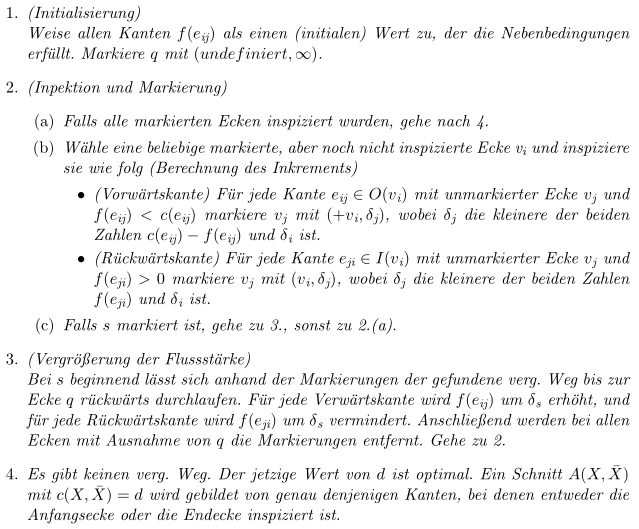
\includegraphics[height=6.8cm]{../algorithmus.PNG}
        \end{center}
    \end{frame}

    \begin{frame}{Kontext - Algorithmen}
        \begin{block}{Besonderheiten}
            \begin{itemize}
                \item \textbf{Ford-Fulkerson} und \textbf{Edmonds-Karp} unterscheiden sich nur in der Suchreihenfolge nach einem vergr. Weg.
                \item \textbf{Edmonds-Karp} verwendet hierzu eine \textit{Queue}
                \item Durch den spezifizierten R\"uckgabewert\\
                $[($\textit{Liste der im letzten Lauf inspizierten Knoten}$)]$\\
                kann Schritt 4. der Algorithmen vernachl\"assigt werden
            \end{itemize}
        \end{block}
    \end{frame}

    \begin{frame}{Kontext - Komplexit\"at}
        \begin{block}{aus 1. \textit{(Initialisierung)}}
            \begin{itemize}
                \item Setzen von Werten: \textit{O(1)}
                \item Iterieren von Kanten: \textit{O(N)}
            \end{itemize}
        \end{block}
        \begin{block}{aus 2. \textit{(Inspektion und Markierung)}}
            \begin{itemize}
                \item Markierung/Inspektion pr\"ufen: \textit{O(1)}
                \item Iterieren von Knoten: \textit{O(N)}
            \end{itemize}
        \end{block}
    \end{frame}

    \begin{frame}{Kontext - Komplexit\"at}
        \begin{block}{aus 2. (b)}
            \begin{itemize}
                \item W\"ahlen einer beliebigen Ecke: \textit{O(N)}
                \item W\"ahlen der n\"achsten Ecke aus der Queue: \textit{O(1)}
                \item Inzidente Kanten abfragen: \textit{O(1)}
            \end{itemize}
        \end{block}

        \begin{block}{Erwartete Komplexit\"at}
            \begin{itemize}
                \item \textit{O(Anzahl Kanten x Maximale Anzahl an vergr. Wegen)}
                \item \textit{O(Anzahl Knoten x Anzahl Kanten x Anzahl Kanten)}
            \end{itemize}
        \end{block}
    \end{frame}

    \section{Entwurf}
    \begin{frame}{Entwurf}
        \begin{block}{Definition}
            \begin{itemize}
                \item Alleinige Vorlage zu einer m\"oglichen Implementierung unabh\"agig zur Programmiersprache
                \item M\"ogliche Probleme schnell erkennen, um Aufwand zu minimieren
                \item Grundlegendes f\"ur effiziente Implementierungen und damit gute Softwarel\"osungen schaffen
            \end{itemize}
        \end{block}
    \end{frame}

    \begin{frame}{Entwurf - Algorithmen}
        \begin{block}{Wirkungsprinzip}
            \begin{center}
                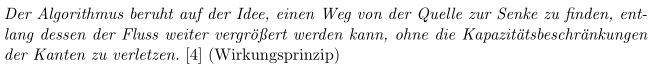
\includegraphics[width=10.8cm]{../wirkungsprinzip.PNG}
            \end{center}
        \end{block}

        \begin{block}{Informationen an Ecken und Kanten}
            \begin{itemize}
                \item Ecken: $(+/-$,Vorg\"anger,$\delta)$
                \item Kanten: Fluss, Kapazit\"at
            \end{itemize}
        \end{block}
    \end{frame}

    \begin{frame}{Entwurf - Datenstrukturen}
        \begin{block}{Allgemein}
            Effiziente Organisation von Daten mit Listen und Tupeln
        \end{block}
        \begin{block}{aus 1. \textit{(Initialisierung)}}
            \begin{itemize}
                \item Setzen eines initialen Flusses durch rekursives Durchlaufen aller Kanten
            \end{itemize}
        \end{block}
        \begin{block}{aus 2. \textit{(Inspektion und Markierung)}}
            \begin{itemize}
                \item Knoten werden durch die Informationen "`Vorzeichen"', "`Vorg\"anger"' und "`Delta"' markiert
                \item Knoten werden inspiziert
            \end{itemize}
        \end{block}
    \end{frame}

    \begin{frame}{Entwurf - Datenstrukturen}
        \begin{block}{aus 2. (b)}
            \begin{itemize}
                \item Ermitteln einer beliebigen Ecke / Holen einer Ecke aus der Queue
                \item Holen der Inzidenten Kanten der Ecke
            \end{itemize}
        \end{block}

        \begin{block}{aus 2. \textit{(Vergr\"o\ss{}erung der Flussst\"arke)}}
            \begin{itemize}
                \item Knoten der L\"aufe von Vergr\"o\ss{}erung sind zu halten (R\"uckgabewert)
            \end{itemize}
        \end{block}
    \end{frame}

    \begin{frame}{Entwurf - Programmfluss}
        \begin{center}
            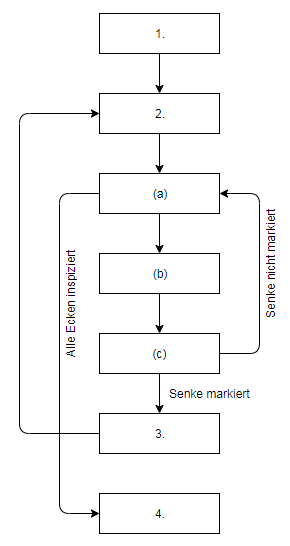
\includegraphics[width=3.6cm]{../fordfulkerson.PNG}
        \end{center}
    \end{frame}

    \section{Laufzeitmessung}
    \begin{frame}{Laufzeitmessung}
        \begin{block}{Idee}
            \begin{itemize}
                \item[I.] Untersuchung bei steigender maximaler Kapazit\"at
                \item[II.] Untersuchung bei steigender Anzahl an Knoten und Kanten
            \end{itemize}
        \end{block}

        \begin{block}{Zusatz}
            \begin{itemize}
                \item Nutzen von \textbf{gengraph} zur Erstellung randomisierter Graphen f\"ur Laufzeitexperimente
            \end{itemize}
        \end{block}
    \end{frame}

    \begin{frame}{Laufzeitmessung - Versuchsaufbau}
        \begin{block}{Parameter}
            \begin{itemize}
                \item Anzahl Ecken
                \item minimaler Grad
                \item maximaler Grad
                \item Mindestgewicht
                \item Maximalgewicht
            \end{itemize}
        \end{block}
    \end{frame}

    \begin{frame}{Laufzeitmessung - Versuch 1}
        \begin{block}{Maximale Kapazit\"at}
            \begin{itemize}
                \item Schrittweise Erh\"ohung der maximalen Kapazit\"at
                \item Konstante Restparameter
            \end{itemize}
        \end{block}

        \begin{block}{Erwartung}
            \begin{itemize}
                \item Ausrei\ss{}er in der Laufzeit beim \textbf{Ford-Fulkerson}
                \item Konstanter \textbf{Edmonds-Karp}
            \end{itemize}
        \end{block}
    \end{frame}

    \begin{frame}{Laufzeitmessung - Versuch 1}
        \begin{center}
            \begin{tabular}{c|c|c|c}
                Messung & \textbf{Edmonds-Karp} & \textbf{Ford-Fulkerson} & Maximale Kapazit\"at\\
                \hline
%                942 & 753 & 10\\
%                989 & 930 & 20\\
%                1056 & 1054 & 30\\
%                1054 & 839 & 40\\
%                1061 & 1080 & 50\\
%                1064 & 826 & 60\\
%                1034 & 974 & 70\\
%                1062 & 1140 & 80\\
%                1077 & 878 & 90\\
%                1028 & 879 & 100\\
                1. & 942 & 753 & 10\\
                2. & 989 & 930 & 20\\
                3. & 1056 & 1054 & 30\\
                4. & 1054 & 839 & 40\\
                5. & 1061 & 1080 & 50\\
                6. & 1064 & 826 & 60\\
                7. & 1034 & 974 & 70\\
                8. & 1062 & 1140 & 80\\
                9. & 1077 & 878 & 90\\
                10. & 1028 & 879 & 100\\
            \end{tabular}
        \end{center}
    \end{frame}

    \begin{frame}{Laufzeitmessung - Versuch 1}
        \begin{center}
            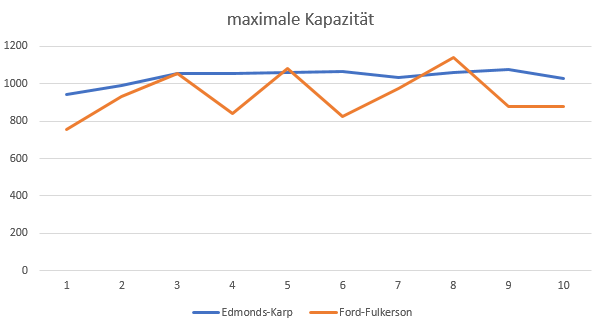
\includegraphics[width=10cm]{../max-capacity-graph.PNG}
        \end{center}
    \end{frame}

    \begin{frame}{Laufzeitmessung - Versuch 1}
        \begin{block}{Auswertung}
            \begin{itemize}
                \item Erwartete Laufzeit
            \end{itemize}
        \end{block}
    \end{frame}

    \begin{frame}{Laufzeitmessung - Versuch 2}
        \begin{block}{Anzahl Ecken und Kanten}
            \begin{itemize}
                \item Schrittweise Erh\"ohung der Anzahl Ecken und Kanten
                \item Konstante Restparameter
                \item maximale Kapazit\"at von 1
            \end{itemize}
        \end{block}

        \begin{block}{Erwartung}
            \begin{itemize}
                \item Laufzeit von \textit{O(E*V)} bei beiden Algorithmen
            \end{itemize}
        \end{block}
    \end{frame}

    \begin{frame}{Laufzeitmessung - Versuch 2}
        \begin{center}
            \begin{tabular}{c|c|c|c}
                Messung & \textbf{Edmonds-Karp} & \textbf{Ford-Fulkerson} & Anzahl Ecken (Kanten)\\
                \hline
                1. & 6311 & 8201 & 105 (5460)\\
                2. & 7744 & 9850 & 110 (5995)\\
                3. & 9113 & 11732 & 115 (6555)\\
                4. & 10960 & 13925 & 120 (7140)\\
                5. & 13108 & 16321 & 125 (7750)\\
                6. & 15135 & 18698 & 130 (8385)\\
                7. & 17626 & 21771 & 135 (9045)\\
                8. & 20338 & 25076 & 140 (9730)\\
                9. & 23257 & 28715 & 145 (10440)\\
                10. & 26562 & 32950 & 150 (11175)\\
            \end{tabular}
        \end{center}
    \end{frame}

    \begin{frame}{Laufzeitmessung - Versuch 2}
        \begin{center}
            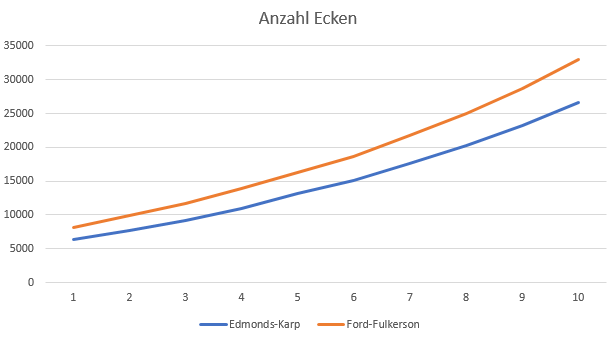
\includegraphics[width=10cm]{../anzahl-kanten-graph.PNG}
        \end{center}
    \end{frame}

    \begin{frame}{Laufzeitmessung - Versuch 1}
        \begin{block}{Auswertung}
            \begin{itemize}
                \item Der \textit{Edmonds-Karp} Algorithmus l\"auft effizienter
                \item Nicht die erwartete Laufzeit
                \item Liegt vermutlich an der Initialisierungzeit der Algorithmen
            \end{itemize}
        \end{block}
    \end{frame}

    \begin{frame}{Ende}
        \begin{center}
            Danke f\"ur Ihre Aufmerksamkeit!
        \end{center}
    \end{frame}

    \begin{frame}{Quellen}
        \begin{center}
            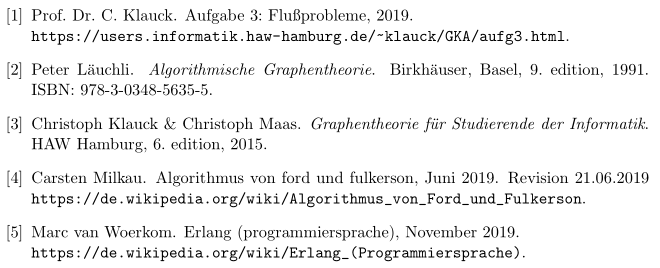
\includegraphics[height=4.4cm]{../quellen.PNG}
        \end{center}
    \end{frame}

\end{document}